\subsection{Fact 3: the FOMC's $r^{*}$ and the econometric $r^{*}$ move in opposite directions}

The FOMC's estimate can be compared against the leading model-based alternative. Holston,
Laubach \& Williams estimate the equilibrium real rate from a semi-structural macro model with a
Kalman filter, quarterly from 1961. Under the martingale assumption in
\S\ref{sec:framework} the two are estimates of the same object: HLW's contemporaneous
$r^{*}_t$ and the FOMC's longer-run projection coincide when $E_t[r^{*}_{t+j}] = r^{*}_t$.

They do not behave like estimates of the same object (Figure~\ref{fig:rstartwo}). Across the 57
SEP meetings the correlation of levels is $\mathbf{-0.93}$.
Between January 2012 and March 2022 the FOMC marked its own $r^{*}$ \emph{down} by 1.78 pp,
from 2.21\% to 0.42\%, while HLW marked $r^{*}$ \emph{up} by 1.37 pp, from 0.89\% to a peak of
2.26\%. After 2022 they swap: the FOMC revises up 0.74 pp while HLW falls back. The two series
cross exactly once, in June 2016, and the mean absolute gap between them is 0.88 pp --- they sit
within 25 bp of each other at only 5\% of meetings.

\begin{figure}[tbp]
\centering
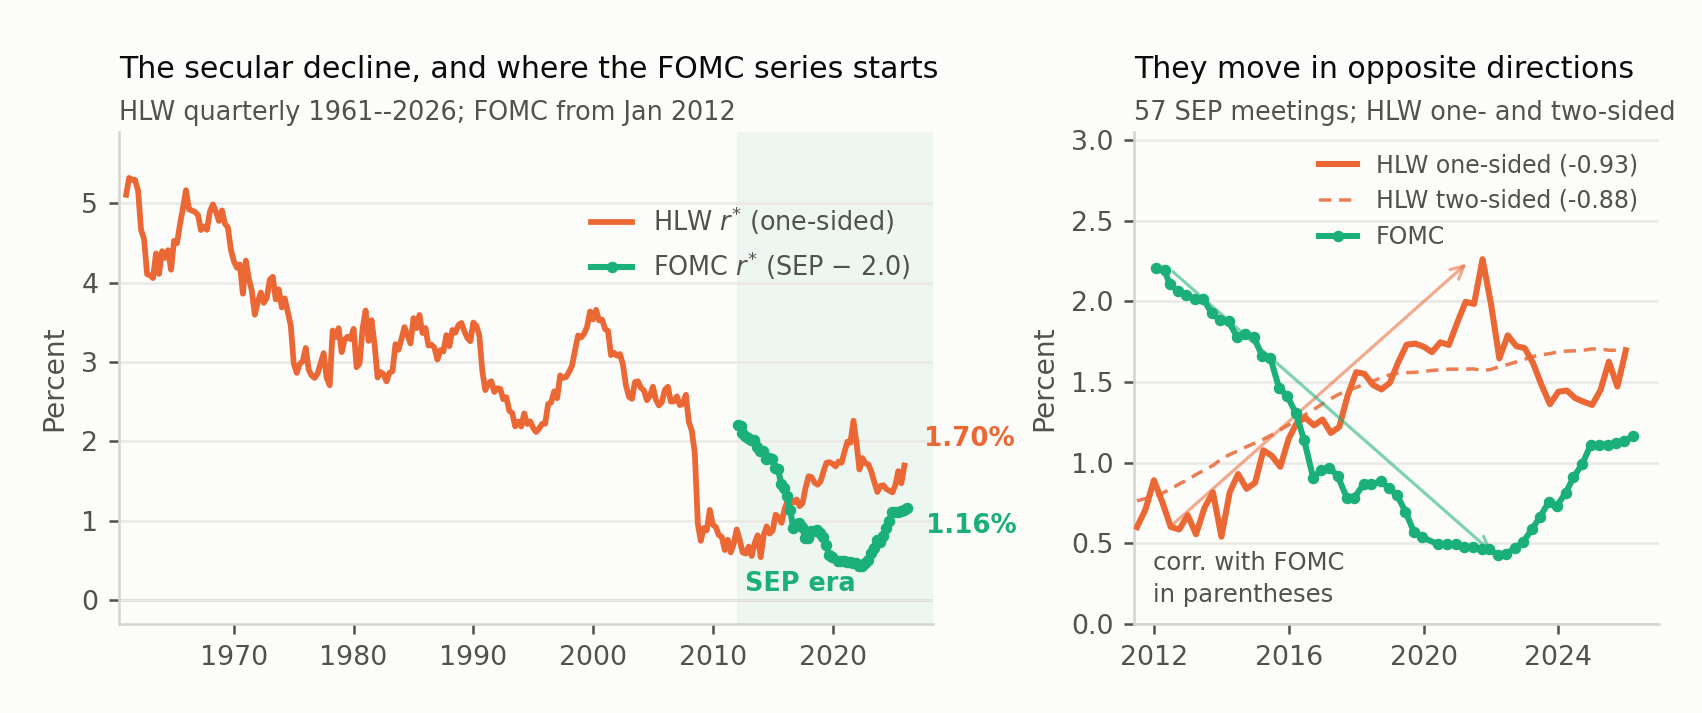
\includegraphics[width=0.95\textwidth]{s_rstar_two.png}
\caption{\textbf{Fact 3.} Left: HLW $r^{*}$ over the full quarterly sample with the FOMC series,
which begins in January 2012, overlaid; the SEP era is shaded. Right: the overlap sample, showing both the one-sided and two-sided
HLW estimates, with arrows marking the direction each series travels over 2012--2022 and the
correlation with the FOMC series in parentheses.}
\label{fig:rstartwo}
\end{figure}

One caveat bounds the reading, and it is narrower than it first appears. The HLW series used
here is the \emph{one-sided} estimate, filtered using data only through each date, so the
comparison is not contaminated by state smoothing; substituting the two-sided estimate leaves
the level correlation at $-0.88$ and makes the correlation of changes more negative, at $-0.36$
(Figure~\ref{fig:rstartwo}, right panel). What remains is vintage: this is the May 2026 release,
so its parameters are estimated on the full sample and its inputs are revised national accounts
data, and a strict real-time comparison would require the historical vintages. The pandemic is
the other concern --- the one-sided series climbs to 2.26\% in 2021 against 1.70\% for the
two-sided --- but neither issue touches 2012--2019, where the two series move steadily apart and
cross.

Three things follow. First, \emph{the Fed's $r^{*}$ is not recoverable from an econometric model}:
if the project needs the Committee's own belief, it has to use the Committee's own publication,
and no model-based series substitutes for it. Second, the same holds for the market side, which
is the third independent reason --- alongside the two in \S\ref{sec:completed} --- that a
model-based endpoint cannot serve as the market leg. Third, and least comfortably for the
mechanism in \S\ref{sec:fact1}, the premise that the Fed holds an information advantage about
$r^{*}$ has an observable consequence: over the decade in which the Committee cut its estimate
by 1.78 pp, the best available econometric estimate moved the other way. Whether the Committee
or the model was closer to right is a question this project does not settle, but it is not a
question the existing literature has posed.
